%%%%%%%%%%%%%%%%%%%%%%%%%%%%%%%%%%%%%%%%%%%%%%%%%%%%%%%%%%%%%%%%%%%%%%
%%                     Inhibition
%%%%%%%%%%%%%%%%%%%%%%%%%%%%%%%%%%%%%%%%%%%%%%%%%%%%%%%%%%%%%%%%%%%%%%

\subsubsection{Glyph: \glyph{Inhibition}}\label{sec:inhibition}
\color{blue}

An inhibition \textbf{negatively}  the strength, or the probability, of the target relationship. This inhibition can be for instance a steric hindrance or a negative allosteric regulation.

\begin{glyphDescription}
 \glyphSboTerm SBO:0000170 ! inhibition.
 \glyphOrigin Any \glyph{entity node} (\sect{ENs}).
 \glyphTarget Any \glyph{relationship} (\sect{relationships}).
 \glyphEndPoint The target extremity of a \glyph{inhibition} carries a bar perpendicular to the arc.
 \end{glyphDescription}

\begin{figure}[H]
  \centering
  \includegraphics[scale = 0.5]{images/inhibition}
  \caption{The \PD glyph for \glyph{inhibition}.}
  \label{fig:inhibition}
\end{figure}

\begin{figure}[H]
  \centering
  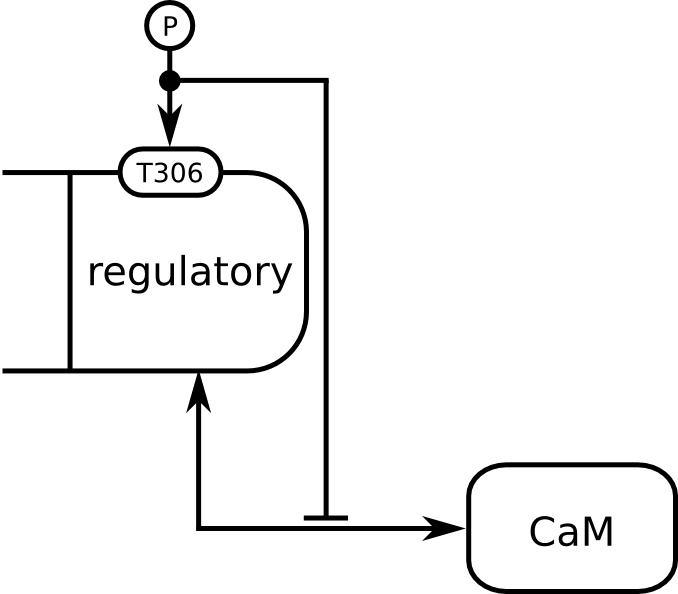
\includegraphics[scale = 0.5]{examples/ex-inhibition}
  \caption{In this example, the phosphorylation of the threonine 306 of the regulatory domain of CaMKII inhibits the interaction between Calmodulin and the kinase.}
  \label{fig:ex-inhibition}
\end{figure}

\normalcolor

